%
% graph.tex -- Graph picture
%
% (c) 2019 Prof Dr Andreas Müller, Hochschule Rapperswil
%
\documentclass[tikz,12pt]{standalone}
\usepackage{amsmath}
\usepackage{times}
\usepackage{txfonts}
\usepackage{pgfplots}
\usepackage{csvsimple}
\usetikzlibrary{arrows,intersections,math}
\begin{document}
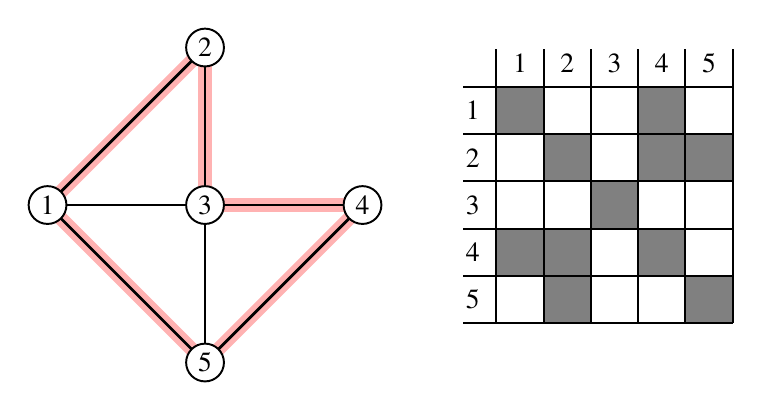
\begin{tikzpicture}[>=latex]

%
% graph-common.tex -- common parts of the graph
%
% (c) 2019 Prof Dr Andreas Müller, Hochschule Rapperswil
%
\coordinate (A1) at (0,0);
\coordinate (A2) at (2,2);
\coordinate (A3) at (2,0);
\coordinate (A4) at (4,0);
\coordinate (A5) at (2,-2);

\def\feld#1#2#3{
	\fill[color=#3] ({#1-0.5},{-#2-0.5}) --({#1+0.5},{-#2-0.5})
		--({#1+0.5},{-#2+0.5}) --({#1-0.5},{-#2+0.5})--cycle;
}

\def\blob#1#2#3{
	\fill[color=#3] (#1,{-#2}) circle[radius=0.4];
}

\begin{scope}[scale=0.8]
\draw[line width=5pt,color=red!30] (A1)--(A2);
\draw[line width=5pt,color=red!30] (A1)--(A5);
\draw[line width=5pt,color=red!30] (A2)--(A3);
\draw[line width=5pt,color=red!30] (A3)--(A4);
\draw[line width=5pt,color=red!30] (A4)--(A5);

\draw[line width=1pt] (A1)--(A2);
\draw[line width=1pt] (A1)--(A3);
\draw[line width=1pt] (A1)--(A5);
\draw[line width=1pt] (A2)--(A3);
\draw[line width=1pt] (A3)--(A4);
\draw[line width=1pt] (A3)--(A5);
\draw[line width=1pt] (A4)--(A5);

\fill[color=white] (A1) circle[radius=0.3];
\fill[color=white] (A2) circle[radius=0.3];
\fill[color=white] (A3) circle[radius=0.3];
\fill[color=white] (A4) circle[radius=0.3];
\fill[color=white] (A5) circle[radius=0.3];

\draw[line width=0.7pt] (A1) circle[radius=0.3];
\draw[line width=0.7pt] (A2) circle[radius=0.3];
\draw[line width=0.7pt] (A3) circle[radius=0.3];
\draw[line width=0.7pt] (A4) circle[radius=0.3];
\draw[line width=0.7pt] (A5) circle[radius=0.3];

\node at (A1) {$1$};
\node at (A2) {$2$};
\node at (A3) {$3$};
\node at (A4) {$4$};
\node at (A5) {$5$};
\end{scope}

\newboolean{rotepunkte}
\setboolean{rotepunkte}{false}

\def\bild{
\begin{scope}[scale=0.6,xshift=9cm,yshift=3cm]
\node at (0,-1) {$1$};
\node at (0,-2) {$2$};
\node at (0,-3) {$3$};
\node at (0,-4) {$4$};
\node at (0,-5) {$5$};
\node at (1,0) {$1$};
\node at (2,0) {$2$};
\node at (3,0) {$3$};
\node at (4,0) {$4$};
\node at (5,0) {$5$};
\feld{1}{1}{gray}
\feld{2}{2}{gray}
\feld{3}{3}{gray}
\feld{4}{4}{gray}
\feld{5}{5}{gray}
\feld{1}{4}{gray}
\feld{4}{1}{gray}
\feld{2}{4}{gray}
\feld{4}{2}{gray}
\feld{2}{5}{gray}
\feld{5}{2}{gray}
\ifthenelse{\boolean{rotepunkte}}{
\blob{2}{1}{red!30}
\blob{1}{2}{red!30}
\blob{3}{2}{red!30}
\blob{2}{3}{red!30}
\blob{4}{3}{red!30}
\blob{3}{4}{red!30}
\blob{5}{4}{red!30}
\blob{4}{5}{red!30}
\blob{5}{1}{red!30}
\blob{1}{5}{red!30}
}{}
\foreach \x in {0.5,1.5,...,5.5}{
\draw[line width=0.7pt] (\x,0.3)--(\x,-5.5);
\draw[line width=0.7pt] (-0.2,{-\x})--(5.5,{-\x});
}
\end{scope}
}

\bild



%\coordinate (A1) at (0,0);
%\coordinate (A2) at (2,2);
%\coordinate (A3) at (2,0);
%\coordinate (A4) at (4,0);
%\coordinate (A5) at (2,-2);
%
%\def\feld#1#2#3{
%	\fill[color=#3] ({#1-0.5},{-#2-0.5}) --({#1+0.5},{-#2-0.5})
%		--({#1+0.5},{-#2+0.5}) --({#1-0.5},{-#2+0.5})--cycle;
%}
%
%\def\blob#1#2#3{
%	\fill[color=#3] (#1,{-#2}) circle[radius=0.4];
%}
%
%
%\begin{scope}[scale=0.8]
%\draw[line width=5pt,color=red!30] (A1)--(A2);
%\draw[line width=5pt,color=red!30] (A1)--(A5);
%\draw[line width=5pt,color=red!30] (A2)--(A3);
%\draw[line width=5pt,color=red!30] (A3)--(A4);
%\draw[line width=5pt,color=red!30] (A4)--(A5);
%
%\draw[line width=1pt] (A1)--(A2);
%\draw[line width=1pt] (A1)--(A3);
%\draw[line width=1pt] (A1)--(A5);
%\draw[line width=1pt] (A2)--(A3);
%\draw[line width=1pt] (A3)--(A4);
%\draw[line width=1pt] (A3)--(A5);
%\draw[line width=1pt] (A4)--(A5);
%
%\fill[color=white] (A1) circle[radius=0.3];
%\fill[color=white] (A2) circle[radius=0.3];
%\fill[color=white] (A3) circle[radius=0.3];
%\fill[color=white] (A4) circle[radius=0.3];
%\fill[color=white] (A5) circle[radius=0.3];
%
%\draw[line width=0.7pt] (A1) circle[radius=0.3];
%\draw[line width=0.7pt] (A2) circle[radius=0.3];
%\draw[line width=0.7pt] (A3) circle[radius=0.3];
%\draw[line width=0.7pt] (A4) circle[radius=0.3];
%\draw[line width=0.7pt] (A5) circle[radius=0.3];
%
%\node at (A1) {$1$};
%\node at (A2) {$2$};
%\node at (A3) {$3$};
%\node at (A4) {$4$};
%\node at (A5) {$5$};
%\end{scope}
%
%\newboolean{rotepunkte}
%\setboolean{rotepunkte}{false}
%
%\def\bild{
%\begin{scope}[scale=0.6,xshift=9cm,yshift=3cm]
%\node at (0,-1) {$1$};
%\node at (0,-2) {$2$};
%\node at (0,-3) {$3$};
%\node at (0,-4) {$4$};
%\node at (0,-5) {$5$};
%\node at (1,0) {$1$};
%\node at (2,0) {$2$};
%\node at (3,0) {$3$};
%\node at (4,0) {$4$};
%\node at (5,0) {$5$};
%\feld{1}{1}{gray}
%\feld{2}{2}{gray}
%\feld{3}{3}{gray}
%\feld{4}{4}{gray}
%\feld{5}{5}{gray}
%\feld{1}{4}{gray}
%\feld{4}{1}{gray}
%\feld{2}{4}{gray}
%\feld{4}{2}{gray}
%\ifthenelse{\boolean{rotepunkte}}{
%\blob{2}{1}{red!30}
%\blob{1}{2}{red!30}
%\blob{3}{2}{red!30}
%\blob{2}{3}{red!30}
%\blob{4}{3}{red!30}
%\blob{3}{4}{red!30}
%\blob{5}{4}{red!30}
%\blob{4}{5}{red!30}
%\blob{5}{1}{red!30}
%\blob{1}{5}{red!30}
%}{}
%\foreach \x in {0.5,1.5,...,5.5}{
%\draw[line width=0.7pt] (\x,0.3)--(\x,-5.5);
%\draw[line width=0.7pt] (-0.2,{-\x})--(5.5,{-\x});
%}
%\end{scope}
%}
%
%\bild
%\setboolean{rotepunkte}{true}
%\begin{scope}[xshift=5cm]
%\bild
%\end{scope}

\end{tikzpicture}
\end{document}

